\section{configobj::Section Class Reference}
\label{classconfigobj_1_1Section}\index{configobj::Section@{configobj::Section}}
Inheritance diagram for configobj::Section::\begin{figure}[H]
\begin{center}
\leavevmode
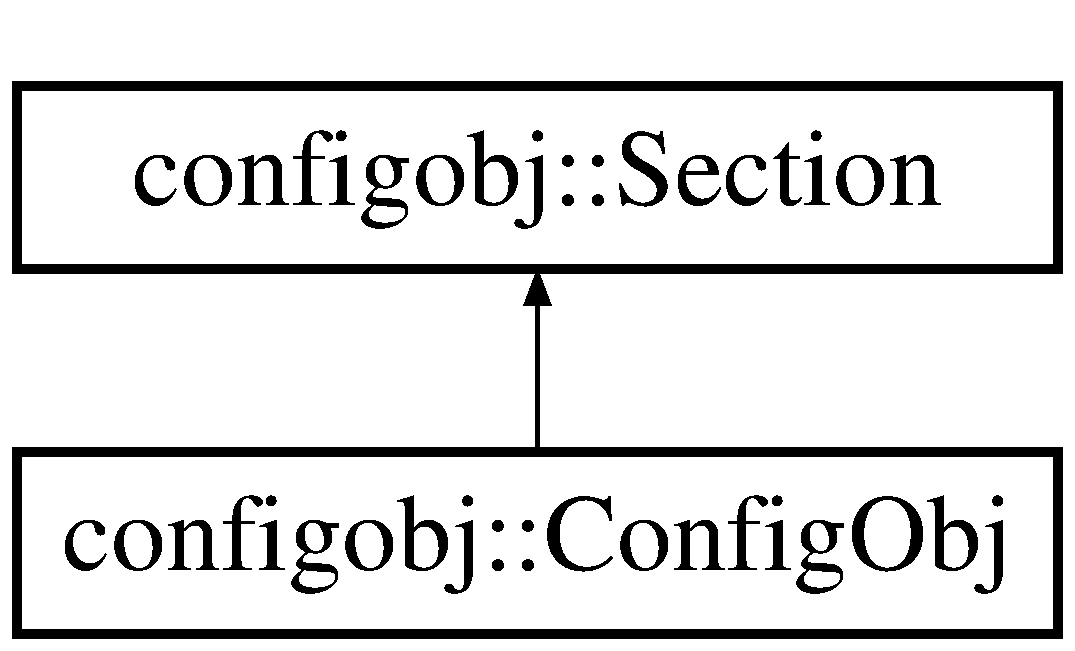
\includegraphics[height=2cm]{classconfigobj_1_1Section}
\end{center}
\end{figure}
\subsection*{Public Member Functions}
\begin{CompactItemize}
\item 
def {\bf\_\-\_\-init\_\-\_\-}
\item 
def {\bf\_\-\_\-getitem\_\-\_\-}
\item 
def {\bf\_\-\_\-setitem\_\-\_\-}
\item 
def {\bf\_\-\_\-delitem\_\-\_\-}
\item 
def {\bfget}
\item 
def {\bfupdate}
\item 
def {\bfpop}
\item 
def {\bfpopitem}
\item 
def {\bfclear}
\item 
def {\bfsetdefault}
\item 
def {\bfitems}
\item 
def {\bfkeys}
\item 
def {\bfvalues}
\item 
def {\bfiteritems}
\item 
def {\bfiterkeys}
\item 
def {\bfitervalues}
\item 
def \textbf{\_\-\_\-repr\_\-\_\-}\label{classconfigobj_1_1Section_5fb3e185aebfd6b94e8f55a3f3d1ceea}

\item 
def {\bfdict}
\item 
def {\bfmerge}
\item 
def {\bfrename}
\item 
def {\bfwalk}
\item 
def {\bfdecode}
\item 
def {\bfencode}
\item 
def {\bfistrue}
\item 
def {\bfas\_\-bool}
\item 
def {\bfas\_\-int}
\item 
def {\bfas\_\-float}
\end{CompactItemize}


\subsection{Detailed Description}


\footnotesize\begin{verbatim}
A dictionary-like object that represents a section in a config file.

It does string interpolation if the 'interpolation' attribute
of the 'main' object is set to True.

Interpolation is tried first from this object, then from the 'DEFAULT'
section of this object, next from the parent and its 'DEFAULT' section,
and so on until the main object is reached.

A Section will behave like an ordered dictionary - following the
order of the ``scalars`` and ``sections`` attributes.
You can use this to change the order of members.

Iteration follows the order: scalars, then sections.
\end{verbatim}
\normalsize
 



\subsection{Member Function Documentation}
\index{configobj::Section@{configobj::Section}!__init__@{\_\-\_\-init\_\-\_\-}}
\index{__init__@{\_\-\_\-init\_\-\_\-}!configobj::Section@{configobj::Section}}
\subsubsection{\setlength{\rightskip}{0pt plus 5cm}def configobj::Section::\_\-\_\-init\_\-\_\- ( {\em self},  {\em parent},  {\em depth},  {\em main},  {\em indict} = {\tt None},  {\em name} = {\tt None})}\label{classconfigobj_1_1Section_104414e2201178fd4bebf34291736fea}




\footnotesize\begin{verbatim}
* parent is the section above
* depth is the depth level of this section
* main is the main ConfigObj
* indict is a dictionary to initialise the section with
\end{verbatim}
\normalsize
 \index{configobj::Section@{configobj::Section}!__getitem__@{\_\-\_\-getitem\_\-\_\-}}
\index{__getitem__@{\_\-\_\-getitem\_\-\_\-}!configobj::Section@{configobj::Section}}
\subsubsection{\setlength{\rightskip}{0pt plus 5cm}def configobj::Section::\_\-\_\-getitem\_\-\_\- ( {\em self},  {\em key})}\label{classconfigobj_1_1Section_8dd2609e5aad758406ca31be54013e36}




\footnotesize\begin{verbatim}Fetch the item and do string interpolation.\end{verbatim}
\normalsize
 \index{configobj::Section@{configobj::Section}!__setitem__@{\_\-\_\-setitem\_\-\_\-}}
\index{__setitem__@{\_\-\_\-setitem\_\-\_\-}!configobj::Section@{configobj::Section}}
\subsubsection{\setlength{\rightskip}{0pt plus 5cm}def configobj::Section::\_\-\_\-setitem\_\-\_\- ( {\em self},  {\em key},  {\em value},  {\em unrepr} = {\tt False})}\label{classconfigobj_1_1Section_8dd4b4b239ea0130ef5ff941e501725b}




\footnotesize\begin{verbatim}
Correctly set a value.

Making dictionary values Section instances.
(We have to special case 'Section' instances - which are also dicts)

Keys must be strings.
Values need only be strings (or lists of strings) if
``main.stringify`` is set.

`unrepr`` must be set when setting a value to a dictionary, without
creating a new sub-section.
\end{verbatim}
\normalsize
 \index{configobj::Section@{configobj::Section}!__delitem__@{\_\-\_\-delitem\_\-\_\-}}
\index{__delitem__@{\_\-\_\-delitem\_\-\_\-}!configobj::Section@{configobj::Section}}
\subsubsection{\setlength{\rightskip}{0pt plus 5cm}def configobj::Section::\_\-\_\-delitem\_\-\_\- ( {\em self},  {\em key})}\label{classconfigobj_1_1Section_44ee2492c48bf2cfe4997089ca1eec2a}




\footnotesize\begin{verbatim}Remove items from the sequence when deleting.\end{verbatim}
\normalsize
 \index{configobj::Section@{configobj::Section}!get@{get}}
\index{get@{get}!configobj::Section@{configobj::Section}}
\subsubsection{\setlength{\rightskip}{0pt plus 5cm}def configobj::Section::get ( {\em self},  {\em key},  {\em default} = {\tt None})}\label{classconfigobj_1_1Section_1a3d744335ce32ea9f647f5c5ae160e8}




\footnotesize\begin{verbatim}A version of ``get`` that doesn't bypass string interpolation.\end{verbatim}
\normalsize
 \index{configobj::Section@{configobj::Section}!update@{update}}
\index{update@{update}!configobj::Section@{configobj::Section}}
\subsubsection{\setlength{\rightskip}{0pt plus 5cm}def configobj::Section::update ( {\em self},  {\em indict})}\label{classconfigobj_1_1Section_87a92164860a49f6e72851e87d92cc80}




\footnotesize\begin{verbatim}
A version of update that uses our ``__setitem__``.
\end{verbatim}
\normalsize
 \index{configobj::Section@{configobj::Section}!pop@{pop}}
\index{pop@{pop}!configobj::Section@{configobj::Section}}
\subsubsection{\setlength{\rightskip}{0pt plus 5cm}def configobj::Section::pop ( {\em self},  {\em key},  {\em args})}\label{classconfigobj_1_1Section_0533bffcf9d10ef5d4520ce651e38665}




\footnotesize\begin{verbatim}\end{verbatim}
\normalsize
 \index{configobj::Section@{configobj::Section}!popitem@{popitem}}
\index{popitem@{popitem}!configobj::Section@{configobj::Section}}
\subsubsection{\setlength{\rightskip}{0pt plus 5cm}def configobj::Section::popitem ( {\em self})}\label{classconfigobj_1_1Section_35e7d107441c970bcec696d6e2169f70}




\footnotesize\begin{verbatim}Pops the first (key,val)\end{verbatim}
\normalsize
 \index{configobj::Section@{configobj::Section}!clear@{clear}}
\index{clear@{clear}!configobj::Section@{configobj::Section}}
\subsubsection{\setlength{\rightskip}{0pt plus 5cm}def configobj::Section::clear ( {\em self})}\label{classconfigobj_1_1Section_1688b24ab8ce906c658e9b97322e1df3}




\footnotesize\begin{verbatim}
A version of clear that also affects scalars/sections
Also clears comments and configspec.

Leaves other attributes alone :
    depth/main/parent are not affected
\end{verbatim}
\normalsize
 \index{configobj::Section@{configobj::Section}!setdefault@{setdefault}}
\index{setdefault@{setdefault}!configobj::Section@{configobj::Section}}
\subsubsection{\setlength{\rightskip}{0pt plus 5cm}def configobj::Section::setdefault ( {\em self},  {\em key},  {\em default} = {\tt None})}\label{classconfigobj_1_1Section_a7d355edde41d9d53841d9067cf22094}




\footnotesize\begin{verbatim}A version of setdefault that sets sequence if appropriate.\end{verbatim}
\normalsize
 \index{configobj::Section@{configobj::Section}!items@{items}}
\index{items@{items}!configobj::Section@{configobj::Section}}
\subsubsection{\setlength{\rightskip}{0pt plus 5cm}def configobj::Section::items ( {\em self})}\label{classconfigobj_1_1Section_2dc9efcd670db60d80f7b5ecb4b73176}




\footnotesize\begin{verbatim}\end{verbatim}
\normalsize
 \index{configobj::Section@{configobj::Section}!keys@{keys}}
\index{keys@{keys}!configobj::Section@{configobj::Section}}
\subsubsection{\setlength{\rightskip}{0pt plus 5cm}def configobj::Section::keys ( {\em self})}\label{classconfigobj_1_1Section_2104f40dfd98abe904faa716497f5b9e}




\footnotesize\begin{verbatim}\end{verbatim}
\normalsize
 \index{configobj::Section@{configobj::Section}!values@{values}}
\index{values@{values}!configobj::Section@{configobj::Section}}
\subsubsection{\setlength{\rightskip}{0pt plus 5cm}def configobj::Section::values ( {\em self})}\label{classconfigobj_1_1Section_b7a0c15d82e82b4a63083604b1cf2d91}




\footnotesize\begin{verbatim}\end{verbatim}
\normalsize
 \index{configobj::Section@{configobj::Section}!iteritems@{iteritems}}
\index{iteritems@{iteritems}!configobj::Section@{configobj::Section}}
\subsubsection{\setlength{\rightskip}{0pt plus 5cm}def configobj::Section::iteritems ( {\em self})}\label{classconfigobj_1_1Section_26824b9a61ec681c2ca79347b2b00dc0}




\footnotesize\begin{verbatim}\end{verbatim}
\normalsize
 \index{configobj::Section@{configobj::Section}!iterkeys@{iterkeys}}
\index{iterkeys@{iterkeys}!configobj::Section@{configobj::Section}}
\subsubsection{\setlength{\rightskip}{0pt plus 5cm}def configobj::Section::iterkeys ( {\em self})}\label{classconfigobj_1_1Section_7a0a273d019e9fe4fb3e4d957c2cd1cd}




\footnotesize\begin{verbatim}\end{verbatim}
\normalsize
 \index{configobj::Section@{configobj::Section}!itervalues@{itervalues}}
\index{itervalues@{itervalues}!configobj::Section@{configobj::Section}}
\subsubsection{\setlength{\rightskip}{0pt plus 5cm}def configobj::Section::itervalues ( {\em self})}\label{classconfigobj_1_1Section_52a9d191ed39cf88e96dbd32bdd9beb0}




\footnotesize\begin{verbatim}\end{verbatim}
\normalsize
 \index{configobj::Section@{configobj::Section}!dict@{dict}}
\index{dict@{dict}!configobj::Section@{configobj::Section}}
\subsubsection{\setlength{\rightskip}{0pt plus 5cm}def configobj::Section::dict ( {\em self})}\label{classconfigobj_1_1Section_06d25e810941ef1c29beed0def612916}




\footnotesize\begin{verbatim}
Return a deepcopy of self as a dictionary.

All members that are ``Section`` instances are recursively turned to
ordinary dictionaries - by calling their ``dict`` method.

>>> n = a.dict()
>>> n == a
1
>>> n is a
0
\end{verbatim}
\normalsize
 \index{configobj::Section@{configobj::Section}!merge@{merge}}
\index{merge@{merge}!configobj::Section@{configobj::Section}}
\subsubsection{\setlength{\rightskip}{0pt plus 5cm}def configobj::Section::merge ( {\em self},  {\em indict})}\label{classconfigobj_1_1Section_c06d7fa9fdd69a29e78fd65a040e5cf2}




\footnotesize\begin{verbatim}
A recursive update - useful for merging config files.

>>> a = '''[section1]
...     option1 = True
...     [[subsection]]
...     more_options = False
...     # end of file'''.splitlines()
>>> b = '''# File is user.ini
...     [section1]
...     option1 = False
...     # end of file'''.splitlines()
>>> c1 = ConfigObj(b)
>>> c2 = ConfigObj(a)
>>> c2.merge(c1)
>>> c2
{'section1': {'option1': 'False', 'subsection': {'more_options': 'False'}}}
\end{verbatim}
\normalsize
 \index{configobj::Section@{configobj::Section}!rename@{rename}}
\index{rename@{rename}!configobj::Section@{configobj::Section}}
\subsubsection{\setlength{\rightskip}{0pt plus 5cm}def configobj::Section::rename ( {\em self},  {\em oldkey},  {\em newkey})}\label{classconfigobj_1_1Section_afc97b84624c87ecfae890958dc9681d}




\footnotesize\begin{verbatim}
Change a keyname to another, without changing position in sequence.

Implemented so that transformations can be made on keys,
as well as on values. (used by encode and decode)

Also renames comments.
\end{verbatim}
\normalsize
 \index{configobj::Section@{configobj::Section}!walk@{walk}}
\index{walk@{walk}!configobj::Section@{configobj::Section}}
\subsubsection{\setlength{\rightskip}{0pt plus 5cm}def configobj::Section::walk ( {\em self},  {\em function},  {\em raise\_\-errors} = {\tt True},  {\em call\_\-on\_\-sections} = {\tt False},  {\em keywargs})}\label{classconfigobj_1_1Section_388e6c9ae458cd8bc2fac634e9bbc9bd}




\footnotesize\begin{verbatim}
Walk every member and call a function on the keyword and value.

Return a dictionary of the return values

If the function raises an exception, raise the errror
unless ``raise_errors=False``, in which case set the return value to
``False``.

Any unrecognised keyword arguments you pass to walk, will be pased on
to the function you pass in.

Note: if ``call_on_sections`` is ``True`` then - on encountering a
subsection, *first* the function is called for the *whole* subsection,
and then recurses into it's members. This means your function must be
able to handle strings, dictionaries and lists. This allows you
to change the key of subsections as well as for ordinary members. The
return value when called on the whole subsection has to be discarded.

See  the encode and decode methods for examples, including functions.

.. caution::

    You can use ``walk`` to transform the names of members of a section
    but you mustn't add or delete members.

>>> config = '''[XXXXsection]
... XXXXkey = XXXXvalue'''.splitlines()
>>> cfg = ConfigObj(config)
>>> cfg
{'XXXXsection': {'XXXXkey': 'XXXXvalue'}}
>>> def transform(section, key):
...     val = section[key]
...     newkey = key.replace('XXXX', 'CLIENT1')
...     section.rename(key, newkey)
...     if isinstance(val, (tuple, list, dict)):
...         pass
...     else:
...         val = val.replace('XXXX', 'CLIENT1')
...         section[newkey] = val
>>> cfg.walk(transform, call_on_sections=True)
{'CLIENT1section': {'CLIENT1key': None}}
>>> cfg
{'CLIENT1section': {'CLIENT1key': 'CLIENT1value'}}
\end{verbatim}
\normalsize
 \index{configobj::Section@{configobj::Section}!decode@{decode}}
\index{decode@{decode}!configobj::Section@{configobj::Section}}
\subsubsection{\setlength{\rightskip}{0pt plus 5cm}def configobj::Section::decode ( {\em self},  {\em encoding})}\label{classconfigobj_1_1Section_692aaec5d4c624794a3828a2f285225a}




\footnotesize\begin{verbatim}
Decode all strings and values to unicode, using the specified encoding.

Works with subsections and list values.

Uses the ``walk`` method.

Testing ``encode`` and ``decode``.
>>> m = ConfigObj(a)
>>> m.decode('ascii')
>>> def testuni(val):
...     for entry in val:
...         if not isinstance(entry, unicode):
...             print >> sys.stderr, type(entry)
...             raise AssertionError, 'decode failed.'
...         if isinstance(val[entry], dict):
...             testuni(val[entry])
...         elif not isinstance(val[entry], unicode):
...             raise AssertionError, 'decode failed.'
>>> testuni(m)
>>> m.encode('ascii')
>>> a == m
1
\end{verbatim}
\normalsize
 \index{configobj::Section@{configobj::Section}!encode@{encode}}
\index{encode@{encode}!configobj::Section@{configobj::Section}}
\subsubsection{\setlength{\rightskip}{0pt plus 5cm}def configobj::Section::encode ( {\em self},  {\em encoding})}\label{classconfigobj_1_1Section_c516f79e00151a857425a08295c017fa}




\footnotesize\begin{verbatim}
Encode all strings and values from unicode,
using the specified encoding.

Works with subsections and list values.
Uses the ``walk`` method.
\end{verbatim}
\normalsize
 \index{configobj::Section@{configobj::Section}!istrue@{istrue}}
\index{istrue@{istrue}!configobj::Section@{configobj::Section}}
\subsubsection{\setlength{\rightskip}{0pt plus 5cm}def configobj::Section::istrue ( {\em self},  {\em key})}\label{classconfigobj_1_1Section_fc6d42977c16329475dd3e7d068e1b38}




\footnotesize\begin{verbatim}A deprecated version of ``as_bool``.\end{verbatim}
\normalsize
 \index{configobj::Section@{configobj::Section}!as_bool@{as\_\-bool}}
\index{as_bool@{as\_\-bool}!configobj::Section@{configobj::Section}}
\subsubsection{\setlength{\rightskip}{0pt plus 5cm}def configobj::Section::as\_\-bool ( {\em self},  {\em key})}\label{classconfigobj_1_1Section_8dc2258e3f064401b42543b683e9ba36}




\footnotesize\begin{verbatim}
Accepts a key as input. The corresponding value must be a string or
the objects (``True`` or 1) or (``False`` or 0). We allow 0 and 1 to
retain compatibility with Python 2.2.

If the string is one of  ``True``, ``On``, ``Yes``, or ``1`` it returns 
``True``.

If the string is one of  ``False``, ``Off``, ``No``, or ``0`` it returns 
``False``.

``as_bool`` is not case sensitive.

Any other input will raise a ``ValueError``.

>>> a = ConfigObj()
>>> a['a'] = 'fish'
>>> a.as_bool('a')
Traceback (most recent call last):
ValueError: Value "fish" is neither True nor False
>>> a['b'] = 'True'
>>> a.as_bool('b')
1
>>> a['b'] = 'off'
>>> a.as_bool('b')
0
\end{verbatim}
\normalsize
 \index{configobj::Section@{configobj::Section}!as_int@{as\_\-int}}
\index{as_int@{as\_\-int}!configobj::Section@{configobj::Section}}
\subsubsection{\setlength{\rightskip}{0pt plus 5cm}def configobj::Section::as\_\-int ( {\em self},  {\em key})}\label{classconfigobj_1_1Section_4b13bb3a9ecb2478305424696b3f06e1}




\footnotesize\begin{verbatim}
A convenience method which coerces the specified value to an integer.

If the value is an invalid literal for ``int``, a ``ValueError`` will
be raised.

>>> a = ConfigObj()
>>> a['a'] = 'fish'
>>> a.as_int('a')
Traceback (most recent call last):
ValueError: invalid literal for int(): fish
>>> a['b'] = '1'
>>> a.as_int('b')
1
>>> a['b'] = '3.2'
>>> a.as_int('b')
Traceback (most recent call last):
ValueError: invalid literal for int(): 3.2
\end{verbatim}
\normalsize
 \index{configobj::Section@{configobj::Section}!as_float@{as\_\-float}}
\index{as_float@{as\_\-float}!configobj::Section@{configobj::Section}}
\subsubsection{\setlength{\rightskip}{0pt plus 5cm}def configobj::Section::as\_\-float ( {\em self},  {\em key})}\label{classconfigobj_1_1Section_3f13d36392963c5e215b810711f9f8c2}




\footnotesize\begin{verbatim}
A convenience method which coerces the specified value to a float.

If the value is an invalid literal for ``float``, a ``ValueError`` will
be raised.

>>> a = ConfigObj()
>>> a['a'] = 'fish'
>>> a.as_float('a')
Traceback (most recent call last):
ValueError: invalid literal for float(): fish
>>> a['b'] = '1'
>>> a.as_float('b')
1.0
>>> a['b'] = '3.2'
>>> a.as_float('b')
3.2000000000000002
\end{verbatim}
\normalsize
 

The documentation for this class was generated from the following file:\begin{CompactItemize}
\item 
old/PANICtool-1.0/configobj.py\end{CompactItemize}
